%main for analyse

\part{System Analysis}
\label{system_analysis}

\chapter{Description of Water Supply Systems}
\label{description_of_water_supply_systems}

 \emph{This chapter gives a general overview of hydraulic systems and an introduction to the WSS in Randers. The basic topology and structures of water supply networks are explained. Furthermore, the basic components of hydraulic systems are discussed and the unit called head, as an alternative measure of pressure, is introduced.}

\section{Hydraulic system overview}
\label{hydraulic_system_overview}

WSSs are designed to deliver water to consumers in terms of sufficient pressure and appropriate chemical composition. Distribution systems as such are typically transport water from one geographical place to another. In practice, there are different methods existing to achieve this water transport. One example is to make use of natural advantages such as the water stored in mountains, and thereby use the potential energy of the water to provide pressure in the network. Examples for this are countries like Norway and Sweden where the advantages of the landscape are being exploited. However, in this project the source of the water is considered as groundwater, considering that in Denmark all reservoirs in the network are tapping water from the ground. After tapping the water, it goes through a cleaning process at the waterworks and afterwards the pure water is pumped into the network \cite{prahata}. In WSSs, pumps and valves are the elements that enable the delivery of water to the consumers or to elevated reservoirs, storing water for later use. Such a network is illustrated in the figure below: 

%illustration of WSS
\begin{figure}[H]
\centering

\includegraphics[width=0.35\textwidth]{report/pictures/missingfigure}
\caption{Illustration of a WSS.}
\label{fig:WSS_example}
\end{figure}

The delivered water needs to fulfil a certain pressure criteria in order to reach consumers at higher levels. For example, in some cases the pressure has to be high enough to make it to the fourth floor of a building and still provide appropriate pressure in the water taps. Generally, in such cases booster pumps are placed in the area, helping to supply the pressure. Too large pressure values, however increase water losses due to pipe waste \cite{walski2003advanced}.

Another criteria is that the flow through particular pipes need to stay within acceptable limits. A low flow rate can lead to water quality problems due to the undesirable microorganisms in the water and due to the metal and salt accumulation on the wall of the pipes \cite{walski2003advanced}. 

As can be seen in \figref{fig:WSS_example}, typically WSSs consist of pipe, valve, reservoir, elevated reservoir(tank) and pump components. The common property of them is that they are all two-terminal components, therefore they can be characterized by the dynamic relationship between the pressure drop across their two corresponding endpoints and the flow through them \cite{master_aau}. 

\subsection{Pipe networks}
\label{pipe_networks}

Pipes are the most common components of WSSs since they are used for carrying pressurized water. They serve as a connection between components. Normally, the pipe network can be split into different sub-parts, taking into account the physical characteristics and the attributes of the pipes. Therefore, water supply networks can consist of transmission mains, arterial mains, distribution mains and service lines as shown in the example below: 

%illustration of pipe topology / loop configuration
\begin{figure}[H]
\centering
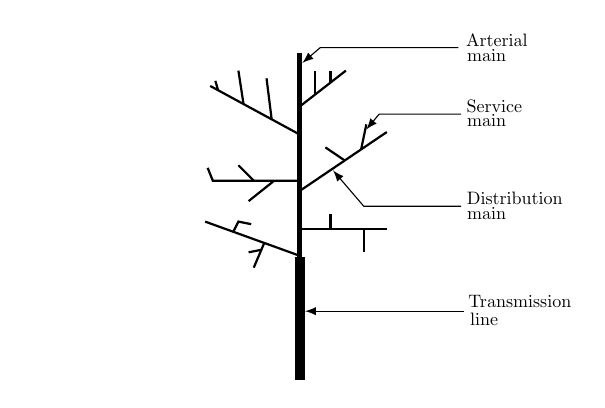
\begin{tikzpicture}[scale=0.65,transform shape]

\fill [black] (0.1,0.1) rectangle (0.3,2.5);
\fill [black] (0.15,6.5) rectangle (0.25,2.5);

\draw [thick](0.15,2.55) -- (-1.65,3.2);
\draw [thick](-0.5,2.77) -- (-0.7,2.3);
\draw [thick](-0.55,2.65) -- (-0.8,2.6);
\draw [thick](-1.1,3) -- (-1,3.2) -- (-0.75,3.15);
\draw [thick](0.2,3.05) -- (1.9,3.05);
\draw [thick](0.8,3.05) -- (0.8,3.35);
\draw [thick](1.45,3.05) -- (1.45,2.6);
\draw [thick](0.2,4) -- (-1.5,4) -- (-1.6,4.25);
\draw [thick](-0.3,4) node (v1) {} -- (-0.8,3.6);
\draw [thick](v1);
\draw [thick](-0.7,4) -- (-1,4.3);
\draw [thick](0.2,3.8) -- (1.9,4.95);
\draw [thick](1.4,4.62) -- (1.5,5.1);
\draw [thick](1.07,4.4) -- (0.7,4.65);
\draw [thick](0.2,4.9) -- (-1.55,5.85);
\draw [thick](-0.35,5.2) -- (-0.45,6);
\draw [thick](-0.9,5.5) -- (-1,6.15);
\draw [thick](-1.4,5.78) -- (-1.45,5.95);
\draw [thick](0.2,5.45) -- (1.1,6.15);
\draw [thick](0.8,5.92) -- (0.8,6.15);
\draw [thick](0.5,5.69) -- (0.5,6.15);
%\draw [-latex](3.4,1.45) -- (0.3,1.85);
\node at (4.5,1.65) {\normalsize Transmission};
\node at (3.8,1.3) {\normalsize line};
%\draw [-latex](3.35,3.4) -- (0.6,4.05);
\node at (4.4,3.65) {\normalsize Distribution};
\node at (3.85,3.35) {\normalsize main};
\node at (4,5.45) {\normalsize Service};
\node at (3.85,5.17) {\normalsize main};
\node at (4.05,6.75) {\normalsize Arterial};
\node at (3.85,6.45) {\normalsize main};
%\draw [-latex](3.25,5.25) -- (1.5,5);
%\draw [-latex](3.2,6.55) -- (0.25,6.4);
\node at (-5,3.6) {         };
\draw [-latex](3.3,6.6) -- (0.6,6.6) -- (0.25,6.3);
\draw [-latex](3.35,5.3) -- (1.75,5.3) -- (1.5,5);
\draw [-latex](3.35,3.5) -- (1.45,3.5) -- (0.85,4.2);
\draw [-latex](3.4,1.45) -- (0.3,1.45);
\end{tikzpicture} 
\caption{Illustration of pipe mains. Tree configuration.}
\label{fig:pipemain_example}
\end{figure}

Transmission mains deliver large amounts of water over long distances. Arterial and distribution mains provide intermediate steps towards delivering water to the end-users. Service lines transmit the water from the distribution mains straight to the end-users \cite{grigg2012water}.

The transmission and distribution network can have a topology that is called a loop or a tree structure. \figref{fig:pipemain_example} shows an example for a tree configuration. This type of configuration is most frequently used in rural areas \cite{mays}. Typically the network has only one path for the water to reach the end-users. Common problems with this configuration is that on the outer parts of the system lower pressures can be experienced due to the pressure losses from long flow paths. The flow dynamics within this kind of systems therefore consist of large flows closer to the source that turn into smaller flows on the outer parts of the system. Main disadvantage of a purely tree structure system is that due to maintenance or momentary breakdowns, the system suffers disruption of service \cite{mays}. 

Loop networks have a configuration as shown in \figref{fig:loop_configuration}. 

%illustration of loop configuration
\begin{figure}[H]
\centering
 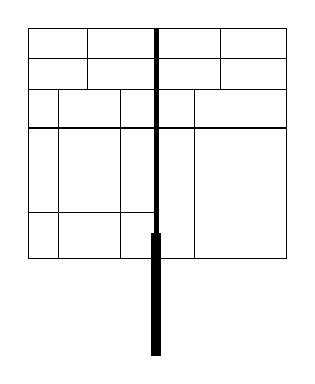
\begin{tikzpicture}[scale=0.65,transform shape]
 
 
\fill [black] (0.1,0.1) rectangle (0.3,2.5);
\fill [black] (0.15,6.5) rectangle (0.25,2.5);


%\node at (-6,3.6) {         };

\draw (0.2,6.5) -- (2.75,6.5) -- (2.75,2) -- (0.3,2);
\draw (0.2,6.5) -- (-2.3,6.5) -- (-2.3,2) -- (0.1,2);
\draw (-2.3,5.3) -- (2.75,5.3);
\draw (-2.3,5.9) -- (2.75,5.9);
\draw (-1.15,6.5) -- (-1.15,5.3);
\draw (1.45,6.5) -- (1.45,5.3);
\draw (-1.7,5.3) -- (-1.7,2);
\draw (-0.5,5.3) -- (-0.5,2);
\draw (-2.3,4.55) -- (0.15,4.55);
\draw (-2.3,2.9) -- (0.15,2.9);
\draw (0.95,5.3) -- (0.95,2);
\draw (0.2,4.55) -- (2.75,4.55);
\end{tikzpicture} 
%
\includegraphics[width=0.35\textwidth]{report/pictures/missingfigure}
\caption{Loop configuration.}
\label{fig:loop_configuration}
\end{figure}

Loop networks are usually composed of smaller loops which made up of smaller distribution mains, and larger loops that are connected to arterial or transmission mains. Elevated reservoirs are typically placed in the centre of the system due to pressure losses resulting from flows through the loop network \cite{council2007drinking}. In the presence of the larger loops, they may be used to feed an internal distribution grid or a distribution grid attached to the outer part of the loop. Loop configurations are generally associated with larger suburban and city distribution systems such as the WSS in Randers\cite{council2007drinking}. 

\subsection{Elevated reservoirs}
\label{elevated_reservoirs}

Elevated reservoirs, or tanks, are typically placed in the system to use them as buffers and level out the pressure and flow demand differences. When the demand is high, the waterworks might not be able to provide the sufficient amount of water in the network. In these cases, the elevated reservoir supplies the remaining demand. When the user consumption decreases, the system can be controlled such that the tank is being refilled to provide the required demand for the next peak time of consumption. Having such an elevated reservoir in the network, the system becomes more independent of the pump stations, as the refilled tank can itself maintain the desired pressure and flow for a limited time. 

Due to the elevation of the tank, when it is filled up, the pumping stations need to provide a pressure higher than the pressure in the water tank. Therefore when the tank is being emptied, the pumping stations can reduce the amount of pressure they provide to the system, since the pressure from the elevated reservoir becomes dominant. This is due to that the dynamics of systems with large storages come primarily from the pressure of the tank \cite{8thsemester_project}. This is due to the height change of the tank being very slow because of the large diameter of the tank. Due to these considerations, the effect of these elevated reservoirs has to be taken into account while modelling the system. 

\subsection{Pumps}
\label{pumps}

Water pumps are used to increase pressure in hydraulic systems, thus making the water flow. Pumps are typically the main actuators of a WSS and they can be either flow or pressure controlled. Therefore, pumps can have controllers to produce a desired flow or pressure. This is done by changing the rotational speed of the pump. In this way, when the pump has a reference pressure or flow, simple control makes it possible to produce the desired flow or pressure respectively \cite{kallesoePHD}.The pressure required to make the water reach some height is the sum of the pressure required to overcome the elevation and the friction losses in the pipe network. 

The most common pumps in WSSs are centrifugal pumps. Normally, the characteristics of such pumps are described by two pump curves. The two curves depict the volume flow versus the pressure and the power of the pump respectively. Normally the curves describe the characteristics for one particular speed, which is denoted the nominal speed \cite{kallesoePHD}. An example of these pump curves is shown in \figref{fig:pump_curves}.

\begin{figure}[H]
\centering
\begin{subfigure}{.49\textwidth}
\centering
  % This file was created by matlab2tikz.
%
%The latest updates can be retrieved from
%  http://www.mathworks.com/matlabcentral/fileexchange/22022-matlab2tikz-matlab2tikz
%where you can also make suggestions and rate matlab2tikz.
%
\definecolor{mycolor1}{rgb}{0.00000,0.44700,0.74100}%
%
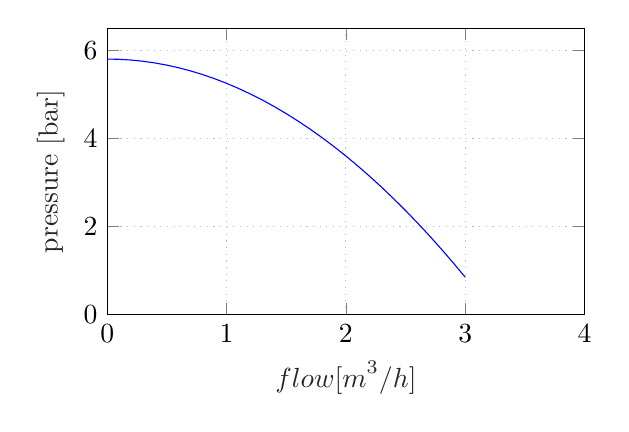
\begin{tikzpicture}

\begin{axis}[%
width=0.5\textwidth,
height=0.3\textwidth,
at={(0.758in,0.499in)},
scale only axis,
xmin=0,
xmax=4,
xlabel style={font=\color{white!15!black}},
xlabel={$\text{flow [m}^\text{3}\text{/h]}$},
ymin=0,
ymax=6.5,
ylabel style={font=\color{white!15!black}},
ylabel={pressure [bar]},
axis background/.style={fill=white},
xmajorgrids,
ymajorgrids,
grid style={dotted}
]
\addplot [color=blue, forget plot]
  table[row sep=crcr]{%
0	5.8\\
0.0999999999999996	5.7945\\
0.2	5.778\\
0.3	5.7505\\
0.4	5.712\\
0.5	5.6625\\
0.600000000000001	5.602\\
0.7	5.5305\\
0.8	5.448\\
0.9	5.3545\\
1	5.25\\
1.1	5.1345\\
1.2	5.008\\
1.3	4.8705\\
1.4	4.722\\
1.5	4.5625\\
1.6	4.392\\
1.7	4.2105\\
1.8	4.018\\
1.9	3.8145\\
2	3.6\\
2.1	3.3745\\
2.2	3.138\\
2.3	2.8905\\
2.4	2.632\\
2.5	2.3625\\
2.6	2.082\\
2.7	1.7905\\
2.8	1.488\\
2.9	1.1745\\
3	0.85\\
};
\end{axis}
\end{tikzpicture}% 
  \caption{Flow versus pressure difference}
  \label{fig:sub1}
\end{subfigure}
\begin{subfigure}{.49\textwidth}
\centering
  % This file was created by matlab2tikz.
%
%The latest updates can be retrieved from
%  http://www.mathworks.com/matlabcentral/fileexchange/22022-matlab2tikz-matlab2tikz
%where you can also make suggestions and rate matlab2tikz.
%
\definecolor{mycolor1}{rgb}{0.00000,0.44700,0.74100}%
%
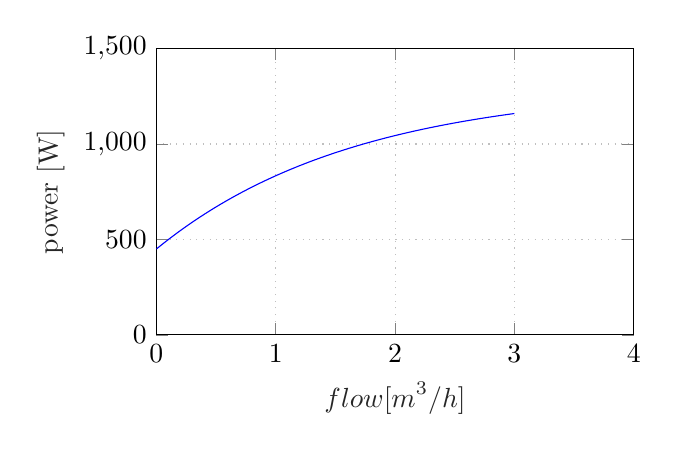
\begin{tikzpicture}

\begin{axis}[%
width=0.5\textwidth,
height=0.3\textwidth,
at={(0.758in,0.499in)},
scale only axis,
xmin=0,
xmax=4,
xlabel style={font=\color{white!15!black}},
xlabel={$\text{flow [m}^\text{3}\text{/h]}$},
ymin=0,
ymax=1500,
ylabel style={font=\color{white!15!black}},
ylabel={power [W]},
axis background/.style={fill=white},
xmajorgrids,
ymajorgrids,
grid style={dotted}
]
\addplot [color=blue, forget plot]
  table[row sep=crcr]{%
0	450\\
0.0599999999999454	480.055750539345\\
0.119999999999891	509.048738560475\\
0.180000000000064	537.01654303413\\
0.240000000000009	563.995414149676\\
0.299999999999955	590.020320300419\\
0.3599999999999	615.124993407542\\
0.420000000000073	639.341972641396\\
0.480000000000018	662.702646596815\\
0.539999999999964	685.237293977134\\
0.599999999999909	706.975122839624\\
0.660000000000082	727.944308453222\\
0.720000000000027	748.172029817625\\
0.779999999999973	767.684504891077\\
0.839999999999918	786.507024572515\\
0.900000000000091	804.663985482109\\
0.960000000000036	822.178921582701\\
1.01999999999998	839.074534683114\\
1.07999999999993	855.372723862874\\
1.1400000000001	871.094613856482\\
1.20000000000005	886.260582434024\\
1.25999999999999	900.890286813621\\
1.31999999999994	915.002689139926\\
1.38000000000011	928.616081061725\\
1.44000000000005	941.74810744047\\
1.5	954.415789220491\\
1.55999999999995	966.635545490521\\
1.61999999999989	978.423214765135\\
1.68000000000006	989.79407551368\\
1.74000000000001	1000.76286596331\\
1.79999999999995	1011.3438032018\\
1.8599999999999	1021.55060160486\\
1.92000000000007	1031.39649061192\\
1.98000000000002	1040.89423187328\\
2.03999999999996	1050.05613579107\\
2.09999999999991	1058.8940774752\\
2.16000000000008	1067.41951213515\\
2.22000000000003	1075.64348992761\\
2.27999999999997	1083.57667027892\\
2.33999999999992	1091.22933570126\\
2.40000000000009	1098.6114051202\\
2.46000000000004	1105.73244673099\\
2.51999999999998	1112.60169040034\\
2.57999999999993	1119.22803962954\\
2.6400000000001	1125.62008309472\\
2.70000000000005	1131.78610577893\\
2.75999999999999	1137.73409971065\\
2.81999999999994	1143.47177432257\\
2.88000000000011	1149.00656644414\\
2.94000000000005	1154.34564994065\\
3	1159.49594501165\\
};
\end{axis}
\end{tikzpicture}% 
  \caption{Flow versus power consumption}
  \label{fig:sub2}
\end{subfigure}
\caption{Pump curves describing the performance of a centrifugal pump at nominal speed.}
\label{fig:pump_curves}
\end{figure}

% %pump curves
% \begin{figure}[H]
% \centering
% % This file was created by matlab2tikz.
%
%The latest updates can be retrieved from
%  http://www.mathworks.com/matlabcentral/fileexchange/22022-matlab2tikz-matlab2tikz
%where you can also make suggestions and rate matlab2tikz.
%
\definecolor{mycolor1}{rgb}{0.00000,0.44700,0.74100}%
%
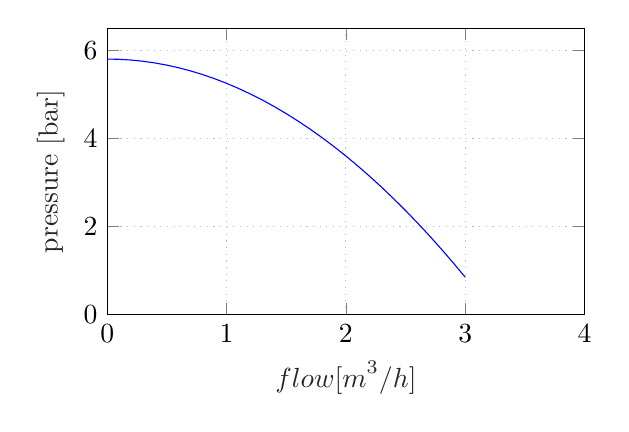
\begin{tikzpicture}

\begin{axis}[%
width=0.5\textwidth,
height=0.3\textwidth,
at={(0.758in,0.499in)},
scale only axis,
xmin=0,
xmax=4,
xlabel style={font=\color{white!15!black}},
xlabel={$\text{flow [m}^\text{3}\text{/h]}$},
ymin=0,
ymax=6.5,
ylabel style={font=\color{white!15!black}},
ylabel={pressure [bar]},
axis background/.style={fill=white},
xmajorgrids,
ymajorgrids,
grid style={dotted}
]
\addplot [color=blue, forget plot]
  table[row sep=crcr]{%
0	5.8\\
0.0999999999999996	5.7945\\
0.2	5.778\\
0.3	5.7505\\
0.4	5.712\\
0.5	5.6625\\
0.600000000000001	5.602\\
0.7	5.5305\\
0.8	5.448\\
0.9	5.3545\\
1	5.25\\
1.1	5.1345\\
1.2	5.008\\
1.3	4.8705\\
1.4	4.722\\
1.5	4.5625\\
1.6	4.392\\
1.7	4.2105\\
1.8	4.018\\
1.9	3.8145\\
2	3.6\\
2.1	3.3745\\
2.2	3.138\\
2.3	2.8905\\
2.4	2.632\\
2.5	2.3625\\
2.6	2.082\\
2.7	1.7905\\
2.8	1.488\\
2.9	1.1745\\
3	0.85\\
};
\end{axis}
\end{tikzpicture}% 
% %
\includegraphics[width=0.35\textwidth]{report/pictures/missingfigure}
% \caption{Loop configuration.}
% \label{fig:pump curves}
% \end{figure}

As can be seen, at a given flow, the pump can deliver a pressure with a maximum limit. This pressure decreases when the flow is increasing. At a certain flow and pressure value, the pump has an optimal point where the operation is the most energy efficient. Pumps are normally designed such that the optimal point lies in the operational area for the pumping application \cite{kenneth_houe}. 

As in almost all WSSs, the flow is varying in the system, according to the flow demand from the end-consumers. Therefore, when dealing with varying flow in the system, pumps are often placed parallel at the pump stations such that they can keep their optimum points. As the flow increases, more pumps get activated to keep the pressure constant \cite{kenneth_houe}. 

\subsection{Valves}
\label{valves}

Valves in the WSS can be also seen as actuators along with pump elements. Unlike the pumps, valves are passive actuators in the sense that they do not consume energy. In principal, there are many types of valves existing. They can be categorized as non-return valves, control valves and the combination of these two. Non-return valves allow waterflow only in one direction, while control valves can either adjust the flow or the pressure on their two endpoints. The former category is typically called a Flow Control Valve(FCV), while the latter is called a Pressure Reducer Valve or Pressure Regulating Valve(PRV). This project deals with all three types of valves. 

Valves can be controlled such that no flow passes through. In these cases the valve is closed and thereby certain parts of the system can be isolated. Other possibility is that the valve is fully open. In such case the pressure drop between the two endpoints is experienced because of the friction loss of the valve. 

\subsection{Hydraulic head}
\label{hydraulic_head}
Since EPANET uses head as the measure of pressure, probably it is more convenient to use head in the report

\section{The Randers water supply network}
\label{the_randers_water_supply_network}

The Randers drinking WSS is managed by Verdo A/S and is the main supplier of drinking water and heating to the city of Randers. Verdo supplies water to approximately 46.000 customers in Randers Municipality \cite{verdo}. The simulation model of the network is illustrated in \figref{fig:reservoirs_epanet}. As can be seen, the WSS in Randers is a complex, looped configuration with many different distribution areas. In overall, the system consists of around 4500 pipe elements, six tanks and more than 20 valves. The water in the network is controlled by eight pumping stations, located at different places throughout the network, thereby making it possible to deliver the desired pressure and flow to the end-users. At these pumping stations, pumps are often placed in parallel connections, due to the reason mentioned in \secref{pumps}. At the outlet of the pumping stations, often PRVs or FCVs are placed. 

Verdo provides the drinking water by drilling from 21 different groundwater bases and has four waterworks for water treatment \cite{verdo}. The geographical position of the reservoirs at these waterworks is shown in \figref{fig:reservoirs_epanet}, encircled in red.   

Missing parts:
\begin{itemize}
  \item Which pump stations are to be controlled
  \item Which tanks 
  \item Why tanks are installed at the place where they are
  \item which distribution areas are (mostly) dependant on which pumping stations - this would be useful to know in order to simplify the network and discard some areas in the network 
\end{itemize}

%illustration of reservoirs in the EPANET model of Randers WSS
\begin{figure}[H]
\centering
 \begin{tikzpicture}[scale=0.65,transform shape]
     \node at (0,0) {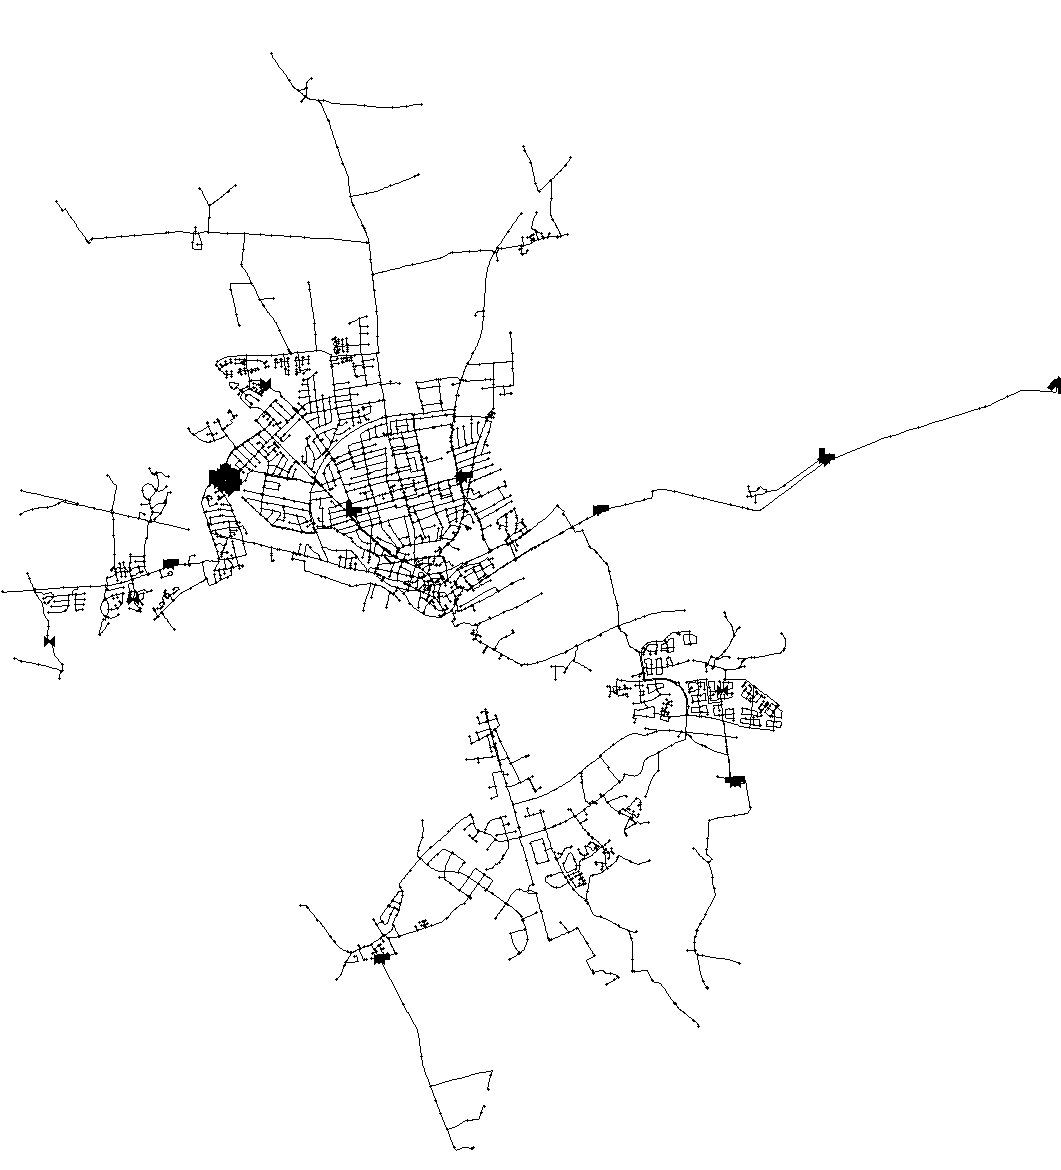
\includegraphics[width=1.5\textwidth]{report/pictures/verdo_pic}};

%     \node[anchor=south west,inner sep=0] at (0,0) {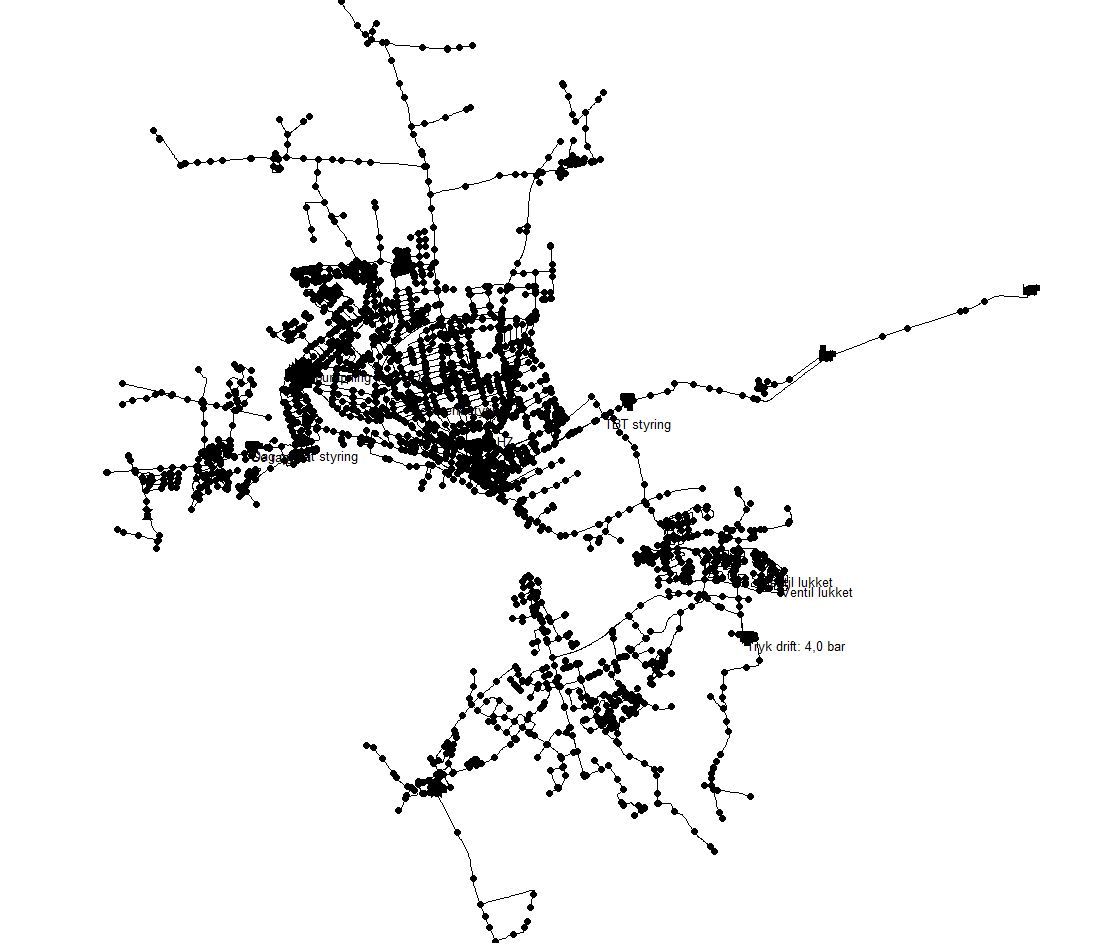
\includegraphics[width=\textwidth]{report/pictures/verdo_pic1}};
            \draw[blue,ultra thick,rounded corners] (3.55,-4.55) rectangle (4.75,-3.7);
             \draw[blue,ultra thick,rounded corners] (5.55,2.15) rectangle (6.8,3);
                      \draw[blue,ultra thick,rounded corners] (-7,2.65) rectangle (-5.75,1.8);
              \draw[blue,line width=0.65mm,rounded corners] (10.05,4.35) rectangle (11.25,3.55);
 \node[black] at (6.05,3.5) {\Large Bunkedal};
   \node[black] at (10.55,4.8) {\Large Østrup Skov};
      \node[black] at (5.6,-4.85) {\Large Vilstrup};
     \node[black] at (-8.55,3) {\Large Oust Mølle};
     
     \draw[red,ultra thick,rounded corners] (-2.1,1.85) rectangle (-0.9,2.7);
      \draw[red,ultra thick,rounded corners] (-8,-0.15) rectangle (-6.8,0.7);
           \draw[red,ultra thick,rounded corners] (1.05,1.15) rectangle (2.25,2);
                \draw[red,ultra thick,rounded corners] (-4.35,1.2) rectangle (-3.15,2.05);
                
                 \node[black] at (2.6,0.65) {\Large Toldbodgade};
                 \node[black] at (0.45,2.85) {\Large Hadsundvej};
                 \node[black] at (-6.45,-0.5) {\Large Hornbæk};
                    \node[black] at (1,5) {\Large Hobrovej};
     
 \draw [-latex](0.1,4.7) -- (-3.25,2.35);
\end{tikzpicture}
 
\caption{Reservoirs in the Randers WSS (encircled in red).}
\label{fig:reservoirs_epanet}
\end{figure}

As can be seen, reservoirs are placed in the outer parts of the city, typically next to the main pumping stations. The locations of the six tanks, or tank stations, in the system is are shown in (figref below)

%illustration of WSS
\begin{figure}[H]
\centering

\includegraphics[width=0.35\textwidth]{report/pictures/missingfigure}
\caption{Illustration of a WSS.}
\label{fig:WSS_example}
\end{figure}



%\section{Setup Considerations}

% This section should contain to things. 

% 1: Req. for water pressure 
% 2: Constrain about water quality 








 
 

\chapter{System Modelling}
\label{system_modelling}

\emph{This chapter gives a mathematical description of the component modelling. Thus the different physical and mathematical measures of hydraulic systems are introduced. The similarities to electronic network modelling are shown by explaining the relevant properties of graph theory. The reduced model for multi-inletsystems is introduced first, then the inclusion of tanks is discussed. In the end, the EPANET-based modelling approach is introduced which is used for simulation purposes within this project.}

\section{Hydraulic component modelling}
\label{hydraulic_component_modelling}

In this section the mathematical relation between pressure and flow is given for each component in a WSS system, in order to show their non-linear behaviour. The purpose here is not to derive the different models, rather to introduce the mathematical formalism which describes them.

\eqref{onecomponent} shows the dual variables which describe all two-terminal components in the network 

\begin{equation}
\label{onecomponent}
 \begin{bmatrix}
    \Delta p \\
    q
\end{bmatrix}
=
 \begin{bmatrix}
    p_{in} - p_{out} \\
    q
\end{bmatrix},
\end{equation}

 \begin{minipage}[t]{0.20\textwidth}
where\\
\hspace*{8mm} $\Delta p$ \\
\hspace*{8mm} $q$ \\
\hspace*{8mm} $p_{in}$, $p_{out}$ 
\end{minipage}
\begin{minipage}[t]{0.68\textwidth}
\vspace*{2mm}
is the differential pressure across the elements,\\
is the flow through the element,\\
are the absolute pressures.
is the flow through the element.
\end{minipage}
\begin{minipage}[t]{0.10\textwidth}
\vspace*{2mm}
\textcolor{White}{te}$\unit{m}$\\
\textcolor{White}{te}$\unit{m}$\\
\textcolor{White}{te}$\unit{\frac{l}{s}}$
\end{minipage}

\subsection{Pipe model}
\label{pipe_component}

Pipes in the network are governed by the dynamic equation

\begin{equation}
\label{complete_pipemodel}
  \Delta p_i = J_i \dot{q_i} + f_i(q_i) - \Delta h_i,
\end{equation}

 \begin{minipage}[t]{0.20\textwidth}
where\\
\hspace*{8mm} $J_i$ \\
\hspace*{8mm} $f_i(q_i)$ \\
\hspace*{8mm} $\Delta h_i$ 
\end{minipage}
\begin{minipage}[t]{0.68\textwidth}
\vspace*{2mm}
is the inertia of the pipes,\\ 
is the pressure drop due to friction,\\
is the pressure drop due to geodesic level difference across the two terminals of pipe elements.
\end{minipage}

The dynamics of the pipes are discarded in the project, as it is shown in other works that the small time constant of the pipe dynamics are not dominant in the system, especially if there are elevated reservoirs included \cite{8thsemester_project,kenneth_houe}. Therefore the pressure across pipes can be written as


\begin{equation}
\label{complete_pipemodel1}
  \Delta p_i = f_i(q_i) - \Delta h_i,
\end{equation}

The pressure drop due to friction across the $i^{th}$ edge is a diagonal map where $f: \mathbb{R}^{m} \rightarrow \mathbb{R}^{m} $ is strictly increasing.\footnote{A map $f: \mathbb{R}^{m} \rightarrow \mathbb{R}^{m} $ is strictly increasing if $\langle x-y, f(x)-f(y) \rangle \geq 0$ for every $x,y \in \: \mathbb{R}^{n}$ such that $x \neq y$ \cite{oneinput_paper}.} As it is shown in \eqref{deltap_friction}, $f_i$ describes a flow dependant pressure drop due to the hydraulic resistance

\begin{equation}
  \label{deltap_friction}
  f_i(q_i) = \rho_i |q_i|q_i,
\end{equation}

 \begin{minipage}[t]{0.20\textwidth}
where\\
\hspace*{8mm} $\rho_i > 0$ 
\end{minipage}
\begin{minipage}[t]{0.68\textwidth}
\vspace*{2mm}
is the parameter of the pipes. 
\end{minipage}

The form in \eqref{deltap_friction} is motivated by turbulent flow in the pipes in the network, which is typical in water supply applications\cite{prahata}. In the following sections it is assumed that each $f_i$ has the structure shown in \eqref{deltap_friction}. 

\subsection{Valve model}
\label{valve_component}

(in progress)

\subsection{Pump model}
\label{pump_component}

(in progress)

\subsection{Elevated reservoir model}
\label{elevatedreservoir_component}

(in progress)

\section{Graph-based network modelling}
\label{graph_based_network_modelling}

Graph-based network modelling has the advantage of making use of tools from circuit theory. Most of these tools are developed based on Graph Theory(GT). These methods can be used to model WSSs as directed graphs, where components of the systems, such as valves, pipes, tanks and pumps correspond to edges and each terminal of the network correspond to nodes, or equivalently, to vertices.

In case of WSSs, in order to track the pressure and flow in the desired part of the network, the equation system of the network has to be solved for the desired edges and vertices. The whole network can be described by writing up the equations for all edges in the network, based on the mathematical modelling of the different components in the system, as shown in \secref{hydraulic_component_modelling}. However, in case of complex systems as water networks for large cities, these systems of equations are hard to handle individually and typically cannot be solved explicitly if there are loops in the system. Therefore the properties of GT are not only useful for setting up relations between flow and pressure, but to make handling of a algebraic constraints easier by exploiting the properties of the matrix representation. Thereby making it convenient for implementing it in computer algorithms for iterative solving methods.  

WSSs can be described by a directed and connected graph, such that \cite{graph_intro}: 

\begin{equation}
  \label{Numberofchords}
  \mathcal{G} = \{\mathcal{V}, \mathcal{E} \} ,
\end{equation}

\begin{minipage}[t]{0.2\textwidth}
where\\
\hspace*{8mm} $\mathcal{G} $ \\
\hspace*{8mm} $\mathcal{V} $ \\
\hspace*{8mm} $\mathcal{E} $
\end{minipage}
\begin{minipage}[t]{0.68\textwidth}
\vspace*{2mm}
is a directed and connected graph,\\
is the set of vertices, where $\mathcal{V} = \{v_1, ..., v_n\}$,\\
is the set of edges, where $\mathcal{E} = \{e_1, ..., e_m\}$. 
\end{minipage}

\subsection{Incidence matrix}
\label{incidence_matrix}

The incidence matrix, $H$, of a connected graph, $\mathcal{G}$, is a matrix where the number of rows and columns correspond to the number of vertices and edges, respectively. Therefore $H\in \: \mathbb{R}^{n \times m}$. In case of hydraulic networks, edges are directed in order to keep track of the direction of the flow in the system. 

\begin{equation}
\label{DiGraph}
 H_{i,j} =
		\left\{
		\begin{array}{ll}
		
		1 			&      \text{if the $j^{th}$ edge is incident out of the $i^{th}$ vertex}.	
\\
	    -1          &      \text{if the $j^{th}$ edge is incident into the $i^{th}$ vertex}.
\\
        0           &      \text{if the $j^{th}$ edge is not connected to the $i^{th}$ vertex}.

		\end{array}
		\right.
\end{equation}	

It is worth mentioning that the reduced incidence matrix can be obtained by removing any arbitrary row from $H$. Therefore $H$ always have $(n-1)$ row rank. This statement can be explained by the mass conservation in the network, which is explained in the following section, \secref{kirchhoffs_law}.

\subsection{Cycle matrix}
\label{cycle_matrix}

Purely tree structure of a WSS is not common when considering water distribution systems. However, trees can be arbitrarily chosen from the underlying graph of the system.\footnote{Recall that a tree with $n$ vertices has $n-1$ edges \cite{deo2017graph}.}  A tree, $\mathcal{T} $, of the graph is a connected sub-graph where any two vertices are connected by exactly one path \cite{deo2017graph}. Therefore a certain sub-graph which is a tree of the network can be represented as follows

\begin{equation}
  \label{Numberofchords}
  \mathcal{T} = \{\mathcal{V_{\mathcal{T}}}, \mathcal{E_{\mathcal{T}}} \} 
\end{equation}

A special case of connected tree sub-graphs is the spanning tree of the network. A spanning tree contains all the vertices of $\mathcal{G}$ and has no cycles, since it is a tree. A spanning tree of the network therefore can be represented as

\begin{equation}
  \label{Numberofchords}
  \mathcal{T} = \{\mathcal{V}, \mathcal{E_{\mathcal{T}}} \} 
\end{equation}

In order to obtain a spanning tree, an edge has to be removed from each cycle. The removed edges are $\mathcal{G} - \mathcal{T}$, and called the chords of $\mathcal{T}$ with respect to $\mathcal{G}$. By adding a chord to $\mathcal{T}$, a cycle is created which is called a fundamental cycle. A graph is conformed by as many fundamental cycles as the number of chords \cite{deo2017graph}.

The set of fundamental cycles correspond to the fundamental cycle matrix, $B$, such that the number of rows and columns are defined by the number of chords and edges, respectively. The cycle matrix of the system is given by

\begin{equation}
\label{DiGraphCycle}
 B_{i,j} =
		\left\{
		\begin{array}{ll}
		
		1 			&     \text{if the $j^{th}$ edge belongs to the $i^{th}$ cycle and their directions agree}	
\\
		-1          &     \text{if the $j^{th}$ edge belongs to the $i^{th}$ cycle and their directions are opposite}
\\
        0           &     \text{if the $j^{th}$ edge does not belong to the $i^{th}$ cycle}
		\end{array}
		\right.
\end{equation}	

\subsection{Kirchhoff's and Ohm's law for hydraulic networks}
\label{kirchhoffs_law}

In this project the hydraulic system is considered to be an open network with pipes, valves, pumps and the storage tanks, where water is able to enter and leave the network at a subset of the vertices. For such a system Kirchhoff's vertex law corresponds to conservation of mass in each vertex and described by

\begin{equation}
  \label{vertexlaw_open}
  Hq = d,
\end{equation}

  \begin{minipage}[t]{0.20\textwidth}
where\\
\hspace*{8mm} $d \in \: \mathbb{R}^{n}$ 
\end{minipage}
\begin{minipage}[t]{0.68\textwidth}
\vspace*{2mm}
is the vector of nodal demands, with $d_i > 0$ when demand flow is into vertex $i$ and $d_i < 0$ when demand flow is out of vertex $i$.
\end{minipage}
\begin{minipage}[t]{0.10\textwidth}
\vspace*{2mm}
\textcolor{White}{te}$\unit{\frac{L}{s}}$
\end{minipage}

Nodal demands can be seen as the end-user consumption, which means that water is taken out from the network. The mass conservation corresponds to the fact that what is consumed from the system must also be produced. Due to mass conservation, there can be only $(n-1)$ independent nodal demands in the network

\begin{equation}
  \label{mass_conservation}
  d_n = - \sum_{i=1}^{n-1} d_i.
\end{equation}

In the further project, a distinction is made between inlet and non-inlet nodes. It is assumed that the demand at non-inlet nodes fulfil the following constraint

\begin{equation}
  \label{non_inlet_constraint}
  d_i \geq 0.
\end{equation}

It is worth noting however, that in closed hydraulic networks the vertex law is

\begin{equation}
  \label{vertexlaw_closed}
  Hq = 0.
\end{equation}

Ohm's law for hydraulic networks therefore can be expressed with the incidence matrix, when $H^T$ is applied to the vector of absolute pressures, $p$. Important to point out that the edges of the underlying graph are considered as only pipe elements

\begin{equation}
  \label{ohmslaw}
  \Delta p = H^Tp = f(q) - H^Th.
\end{equation}

In \eqref{ohmslaw} the differential pressure is described across each edge in the network, taking into account the pressure loss due to friction, $f(q)$ and the pressure drop due to geodesic level differences,  where $h \in \: \mathbb{R}^{n}$ is the vector of geodesic levels at each vertex expressed in units of potential, i.e. pressure. 






\subsection{Multi-inlet reduced network model}
\label{multi_inlet_reduced_network_description}

The system is considered to be a water network supplied from more than one pumping stations and several end-users. In the underlying graph therefore the nodes are pipe connections, with possible water demand from the end-users, and the edges are pipes. The inclusion of storage tanks is the next step of the model development, therefore it is described in a following section, in \secref{inclusion_of_reservoirs}.

The aim of the modelling is to obtain a reduced order network model which is able to capture the dependence of the measured output pressures on the flows and pressures at the inlets. Therefore it is assumed that the inlet pressures and demands are measured. Furthermore, pressure measurement is available in the remaining network, at the end-users. Considering generality, the model is described for $c$ inlets, however it should be noted that regarding the Randers WSS, two inlet points are considered. 

In order to put the system into a form which can handle the measured pressure dependencies on the control inputs, the underlying graph of the network is first partitioned. The $n$ vertices of the graph are separated into two sets

\begin{equation}
  \label{vertices1}
  \mathcal{V} = \{\bar{\mathcal{V}}, \hat{\mathcal{V}} \}, 
\end{equation}

\begin{minipage}[t]{0.3\textwidth}
where\\
\hspace*{8mm} $\hat{\mathcal{V}} = \{\hat{v}_1, ..., \hat{v}_c\}$\\
and \\
\hspace*{8mm} $\bar{\mathcal{V}} = \{\bar{v}_1, ..., \bar{v}_{n-c}\}$ 
\end{minipage}
\begin{minipage}[t]{0.55\textwidth}
\vspace*{2mm}
 represents the vertices corresponding to the inlet points,\\
 represents the remaining vertices in the graph.
\end{minipage}

The partitioning for the $m$ edges of the graph is being chosen such that

\begin{equation}
  \label{edges1}
  \mathcal{E} = \{\mathcal{E_{\mathcal{T}}}, \mathcal{E_{\mathcal{C}}} \},
\end{equation}

\begin{minipage}[t]{0.35\textwidth}
where\\
\hspace*{8mm} $\mathcal{E_{\mathcal{T}}} = \{e_{\mathcal{T},1}, ..., e_{\mathcal{T},n-c}\}$\\
and\\
\hspace*{8mm} $\mathcal{E_{\mathcal{C}}} = \{e_{\mathcal{C},1}, ..., e_{\mathcal{C},m-n+c}\}$. 
\end{minipage}

The subsets regarding edges and the partitioning is chosen such that the sub-matrix, which maps edges in $\mathcal{E_{\mathcal{T}}}$ to vertices in $\bar{\mathcal{V}}$, is invertible. 

Therefore the incidence matrix can be split into four sub-matrices, as shown in \eqref{H_matrix_sub} below

\begin{equation}
\label{H_matrix_sub}
H=
\left[
\begin{array}{c;{2pt/2pt}r}
\bar{H}_{\mathcal{T}} & \bar{H}_{\mathcal{C}} \\
\hdashline[2pt/2pt]
\hat{H}_{\mathcal{T}} & \hat{H}_{\mathcal{C}}
\end{array}
\right],
\end{equation}

\begin{minipage}[t]{0.3\textwidth}
where\\
\hspace*{8mm} $\bar{H}_{\mathcal{T}} \in \mathbb{R}^{(n-c) \times (n-c)}$\\ 
\hspace*{8mm} $\bar{H}_{\mathcal{C}} \in \mathbb{R}^{(n-c) \times (m-n+c)}$\\
\hspace*{8mm} $\hat{H}_{\mathcal{T}} \in \mathbb{R}^{c \times (n-c)}$\\
\hspace*{8mm} $\hat{H}_{\mathcal{C}} \in \mathbb{R}^{c \times (m-n+c)}$
\end{minipage}
\begin{minipage}[t]{0.68\textwidth}
\vspace*{-0.1mm}
is the sub-matrix, mapping edges in $\mathcal{E_{\mathcal{T}}}$ to vertices in $\bar{\mathcal{V}}$,\\ 
is the sub-matrix, mapping edges in $\mathcal{E_{\mathcal{C}}}$ to vertices in $\bar{\mathcal{V}}$,\\
is the sub-matrix, mapping edges in $\mathcal{E_{\mathcal{T}}}$ to vertices in $\hat{\mathcal{V}}$,\\
is the sub-matrix, mapping edges in $\mathcal{E_{\mathcal{C}}}$ to vertices in $\hat{\mathcal{V}}$. 
\end{minipage}

It is worth noting that the only requirement for the edge partitioning is $\bar{H}_{\mathcal{T}}$ being invertible\footnote{$\exists \{\mathcal{V}, \mathcal{E} \} : \bar{H}^{-1}_{\mathcal{T}} \because rank(H) = (n-1) $ \cite{deo2017graph} }. Furthermore, the set $\mathcal{T} = \{\mathcal{V}, \mathcal{E_{\mathcal{T}}} \}$ is not necessarily a tree of the underlying graph, it can be any form of a connected graph that fulfils the requirements. However, one special case is when $c = 1$, meaning that the network has only one inlet. In this case, $\mathcal{T}$ is indeed a spanning tree. 

With the chosen partition, Kirchhoff's vertex law in \eqref{vertexlaw_open} can be rewritten as

\begin{equation}
  \label{vertexlaw_partitioned1}
  \bar{d} = \bar{H}_{\mathcal{T}} q_{\mathcal{T}} + \bar{H}_{\mathcal{C}} q_{\mathcal{C}},
\end{equation}

\begin{equation}
  \label{vertexlaw_partitioned2}
  \hat{d} = \hat{H}_{\mathcal{T}} q_{\mathcal{T}} + \hat{H}_{\mathcal{C}} q_{\mathcal{C}},
\end{equation}

and Ohm's law in \eqref{ohmslaw}, separating the pressure drop due to hydraulic resistance

\begin{equation}
  \label{ohmslaw_partitioned1}
  f_{\mathcal{T}}(q_\mathcal{T}) = \bar{H}^T_{\mathcal{T}} (\bar{p} + \bar{h}) + \hat{H}^T_{\mathcal{T}} (\hat{p} + \hat{h}),
\end{equation}

\begin{equation}
  \label{ohmslaw_partitioned2}
  f_{\mathcal{C}}(q_\mathcal{C}) = \bar{H}^T_{\mathcal{C}} (\bar{p} + \bar{h}) + \hat{H}^T_{\mathcal{C}} (\hat{p} + \hat{h}).
\end{equation}

Writing up \eqref{ohmslaw_partitioned1} and \eqref{ohmslaw_partitioned2} in matrix form

\begin{equation}
\label{ohmslaw_matrixform}
 \begin{bmatrix} 
 f_{\mathcal{T}}(q_\mathcal{T}) \\ 
 f_{\mathcal{C}}(q_\mathcal{C}) 
 \end{bmatrix}
 =
  \underbrace{\begin{bmatrix}
   \bar{H}^T_{\mathcal{T}} & \hat{H}^T_{\mathcal{T}} \\
   \bar{H}^T_{\mathcal{C}} & \hat{H}^T_{\mathcal{C}} 
   \end{bmatrix}}_{\begin{bmatrix} 
                  \bar{H}^T & \hat{H}^T 
                  \end{bmatrix}}
   \begin{bmatrix} 
 (\bar{p} + \bar{h}) \\ 
 (\hat{p} + \hat{h}) 
 \end{bmatrix}
\end{equation}

As it is shown in \eqref{ohmslaw_matrixform}, the transposed incidence matrices can be written up as the two sub-matrices partitioned according to inlet and non-inlet nodes. 

Introducing matrix $B$, in which the arrangement of the edges are the same as for the incidence matrix, $H$, meaning that $B$ is regarding to the graphs $H_{\mathcal{T}}$ and $H_{\mathcal{T}}$. Then $B$ can be given

\begin{equation}
\label{bmatrix}
B
 =
\begin{bmatrix} 
-\bar{H}^T_{\mathcal{C}}\bar{H}^{-T}_{\mathcal{T}} & I 
\end{bmatrix}
\end{equation}

It should be noted that since the set $\mathcal{T}$ does not define a spanning tree when $c>0$, matrix $B$ is not a cycle matrix corresponding to any spanning tree. However, it is defined the same way as cycle matrices are given. For this reason, the following can be written

 \begin{equation}
  \label{meshlaw_analogy}
  BH^T = 
  \begin{bmatrix} 
-\bar{H}^T_{\mathcal{C}}\bar{H}^{-T}_{\mathcal{T}} & I 
\end{bmatrix}
\begin{bmatrix}
   \bar{H}^T_{\mathcal{T}} & \hat{H}^T_{\mathcal{T}} \\
   \bar{H}^T_{\mathcal{C}} & \hat{H}^T_{\mathcal{C}} 
   \end{bmatrix} 
   =
   \begin{bmatrix} 
-\bar{H}^T_{\mathcal{C}}\bar{H}^{-T}_{\mathcal{T}} & I 
\end{bmatrix}
\hat{H}^T.
\end{equation}

It should be noted, that $B \bar{H}^T = 0$ by the definition of matrix $B$ \cite{deo2017graph}. 

Multiplying with B from the left in \eqref{ohmslaw_matrixform} 

\begin{equation}
\label{ohmslaw_matrixform_B}
\begin{bmatrix} 
-\bar{H}^T_{\mathcal{C}}\bar{H}^{-T}_{\mathcal{T}} & I 
\end{bmatrix}
 \begin{bmatrix} 
 f_{\mathcal{T}}(q_\mathcal{T}) \\ 
 f_{\mathcal{C}}(q_\mathcal{C}) 
 \end{bmatrix}
 =
 \begin{bmatrix} 
-\bar{H}^T_{\mathcal{C}}\bar{H}^{-T}_{\mathcal{T}} & I 
\end{bmatrix}
  \begin{bmatrix}
   \bar{H}^T_{\mathcal{T}} & \hat{H}^T_{\mathcal{T}} \\
   \bar{H}^T_{\mathcal{C}} & \hat{H}^T_{\mathcal{C}} 
   \end{bmatrix}
   \begin{bmatrix} 
 (\bar{p} + \bar{h}) \\ 
 (\hat{p} + \hat{h}) 
 \end{bmatrix}
\end{equation}

induces the following expression

\begin{equation}
\label{meshresult}
f_{\mathcal{C}}(q_\mathcal{C}) -\bar{H}^T_{\mathcal{C}}\bar{H}^{-T}_{\mathcal{T}} f_{\mathcal{T}}(q_\mathcal{T}) = (\hat{H}^T_{\mathcal{C}} -\bar{H}^T_{\mathcal{C}}\bar{H}^{-T}_{\mathcal{T}}\hat{H}^T_{\mathcal{T}})(\hat{p} + \hat{h}).
\end{equation}

From \eqref{vertexlaw_partitioned1}, the vector $q_{\mathcal{T}}$, of flows in edges $\mathcal{E}_{\mathcal{T}}$ can be expressed

\begin{equation}
\label{qt_flow}
q_{\mathcal{T}} = -\bar{H}^{-1}_{\mathcal{T}} \bar{H}_{\mathcal{C}} q_\mathcal{C} + \bar{H}^{-1}_{\mathcal{T}} \bar{d}.
\end{equation}

Therefore using \eqref{qt_flow}, \eqref{meshresult} can be rewritten

\begin{equation}
\label{meshresult2}
f_{\mathcal{C}}(q_\mathcal{C}) -\bar{H}^T_{\mathcal{C}}\bar{H}^{-T}_{\mathcal{T}} f_{\mathcal{T}}(-\bar{H}^{-1}_{\mathcal{T}} \bar{H}_{\mathcal{C}} q_\mathcal{C} + \bar{H}^{-1}_{\mathcal{T}} \bar{d}) = (\hat{H}^T_{\mathcal{C}} -\bar{H}^T_{\mathcal{C}}\bar{H}^{-T}_{\mathcal{T}}\hat{H}^T_{\mathcal{T}})(\hat{p} + \hat{h}).
\end{equation} 

Now rewriting the vertex demands at non-inlet vertices, $\bar{d}$, such that

\begin{equation}
\label{noninlet_demand}
\bar{d} = - v \sigma
\end{equation}

  \begin{minipage}[t]{0.20\textwidth}
where\\
\hspace*{8mm} $\bar{d} \in \: \mathbb{R}^{n-c}$\\
\hspace*{8mm} $\sigma \in \: \mathbb{R}_{+}$ \\
\newline
\hspace*{8mm} $v \in \: \mathbb{R}_{n-c}$
\end{minipage}
\begin{minipage}[t]{0.68\textwidth}
\vspace*{2mm}
is the vector of nodal demands in non-inlet vertices,\\
is the total demand in the network, representing the total consumption of the end-users,\\
represents a vector with the property $\sum_{i} v_i = 1 $ and $v_i \in \: (0;1)$.
\end{minipage}



\subsection{Inclusion of elevated reservoirs}
\label{inclusion_of_reservoirs}

As it is described in \eqref{non_inlet_constraint}, a distinction is made between non-inlet and inlet vertices, by assuming that non-inlet vertices have only positive or zero nodal demand. However, when the inclusion of a tank is considered, a special type of node has to be introduced. A node which can have a demand in both positive and negative directions, meaning that the demand is positive when the tank is being filled and negative when it is being emptied.



\section{EPANET modelling}
\label{EPANET_modelling}

EPANET is an open source software, created by the United States Environmental Protection Agency (EPA) for simulating hydraulic networks \cite{agency2016epanet}. EPANET allows to track the flow of water in each pipe, the pressure at each node and the height of water in each tank. Furthermore, it uses a node-based model approach which means that the components in the network are either treated as nodes or links. Valves, pumps, reservoirs and tanks are considered as nodes due to their fixed geographical location and geodesic level. Pipes are considered as the links between the nodes in the network. Therefore, nodes are termination points for one or more pipes. The end-user consumption flow demand is considered as an attribute of certain nodes. Such nodes are called demand nodes and they have a certain water withdrawal. Attributes of nodes in the network are the geographical and geodesic coordinates, the flow demand, the total, and the available head. \cite{agency2016epanet}  

In EPANET, there is a function to carry out simulations within an extended period. Time patterns can be created that make demands at the nodes vary in a periodic way over the course of the time period. Nodal demands, reservoirs and pump schedules can all have time patterns associated with them, thus making the hydraulic simulation of the network more realistic. In order to create a schedule plan for changing reservoir levels or schedules for the pumping strategy, it is sufficient to have simulation data only at certain time steps. Therefore it is sufficient to solve the network using a set of hourly time steps (snapshots) over a period of 24 hours, and use the static, steady-state solutions for pump scheduling \cite{agency2016epanet}. The main function of EPANET is this, and therefore is used within this project for extended period analysis. During the analysis, pressure and flow values, along with the demand pattern can be simulated for periodic time steps. 

Since all nodes and links in the network have their unique IDs, during the project, the name of certain components will always have a reference to the original IDs in EPANET, for the better and clearer trackability. 











\chapter{Network simplification}
\label{network_simplification}

\section{Purpose of the model reduction}
\label{purpose_of_the_model_reduction}

As it is described in \secref{EPANET_modelling}, planning pump schedules and tank level changes in EPANET can be carried out by solving iteratively for long time steps. However, when a complex network is being used for developing different control methods, typically the aim is to find an optimisation method which determines the optimal input to the system. In order to run such an optimizing algorithm on a complex system, the network needs to be solved numerically and several online execution runs are required. 

In case of complex networks with a tree structure, there is only one way from a source node to any node in the system. Therefore the network can be described by solving the equation system of the model explicitly, therefore all pressures can be directly calculated in terms of the flows. In case of loop systems however, the procedure is more dificult, since there is more path to each nodes in the network. The system of equations have to be solved numerically which can dramatically increase the simulation time of an optimization algorithm. The objective of the system reduction and simplification is threfore to reduce the number of network components and especially the loops in the network, such that the accuracy of the simplified model is as close as possible to that of the original network model. 

\section{State of the art model reduction analysis}
\label{state_of_the_art_model_reduction_analysis}

123

\subsection{Simplification of network model components}
\label{simplification of network model components}

Simplification directly, by keeping the basic components but combining and replacing the individual components. (For example, series, parallel pipes. Tree substructure in the system.)

\subsection{Black box simplification}
\label{black_box_simplification}

Replacing the system partially or fully with a system which provides the same function with less complexity. 

\begin{itemize}
  \item static simplification with linearization and simplification
  \item neural network approach 
\end{itemize}























